\subsection{实数的无穷级数与无穷乘积}

有限实数的级数，若它在 R 中收敛，就简称为收敛的。

定义 1. 有限实数的级数称为绝对收敛的，如果其各项的绝对值组成的级数收敛。

命题 4. 有限实数的级数交换收敛当且仅当它绝对收敛。

这由第三章，§ 5，第 7 节，命题 9 以及第 2 节的定理 3 得出。

换句话说，若 \((u_{n})\) 是有限实数的序列，则说通项为 \(u_{n}\) 的级数交换收敛、或说它绝对收敛、或说序列 \((u_{n})\)

在 \(\mathbf{R}\) 中可和，这是一回事。于是第三章 § 5 中证明的可和族的一切性质都可应用于绝对收敛级数。特别地，若通项为 \(u_{n}\) 的级数绝对收敛，则和 \(\sum_{n\in\mathbf{H}} u_{n}\) 对子集 \(\mathbf{H}\) （\(\mathbf{N}\) 的所有子集）存在；又若 \((\mathbf{H}_{p})\) 是 \(\mathbf{N}\) 的一个分拆，我们有

\[
\sum_ {n = 0} ^ {\infty} u _ {n} = \sum_ {p} \left(\sum_ {n \in \mathrm{H} _ {p}} u _ {n}\right)
\]

（绝对收敛级数的结合性）。

正如我们已在第三章 § 5 中指出的，实数级数可以收敛而不交换收敛，即不绝对收敛。

例. 交错级数. 由有限实数的序列 \((u_n)\) 定义的级数称为交错的，如果 \(u_n = (-1)^n v_n\) ，其中 \(v_n \geqslant 0\) 对一切 \(n\) 成立。我们来证明，这类级数收敛的一个充分条件是序列 \((v_n)\) 递减且以 \(0\) 为其极限。因为若 \(s_n\) 表示

\[
\sum_ {p = 0} ^ {n} u _ {p},
\]

\((v_{n})\) 递减这一假设蕴含

\[
s _ {2 n + 1} \leqslant s _ {2 n + 3} \leqslant s _ {2 n + 2} \leqslant s _ {2 n}
\]

对一切 \(n \geqslant 0\) 。序列 \((s_{2n})\) {[}相应地，\((s_{2n+1})\) {]}递减且下有界（相应地，递增且上有界），因此有有限极限 a（相应地，b），且 \(b \leqslant a\) ；由于

\[
a - b = \lim _ {n \rightarrow \infty} (s _ {2 n} - s _ {2 n + 1}) = \lim _ {n \rightarrow \infty} v _ {2 n + 1} = 0,
\]

断言得证。

例如若取 \(v_{n}=1/n\) ，上述条件满足，因此通项为 \((-1)^{n}/n\) 的级数（``交错调和级数''）收敛。我们在第 1 节已看到，通项为 1/n 的级数（``调和级数''）不收敛，从而交错调和级数不绝对收敛。

我们回忆（第三章，§ 5，第 6 节，命题 7）：若 \((u_n)\) 与 \((v_n)\) 是有限实数的两个收敛级数，则级数 \((u_n + v_n)\) 收敛，且

\[
\sum_ {n = 0} ^ {\infty} \left(u _ {n} + v _ {n}\right) = \sum_ {n = 0} ^ {\infty} u _ {n} + \sum_ {n = 0} ^ {\infty} v _ {n};
\]

又，若级数 \((u_{n})\) 收敛，则级数 \((au_{n})\) 对一切有限实数 \(a\) 收敛，且 \(\sum_{n=0}^{\infty} au_{n} = a\) . \(\sum_{n=0}^{\infty} u_{n}\) 。

最后，若级数 \((u_n)\) 与 \((v_n)\) 收敛，且 \(u_n \leqslant v_n\) 对一切 \(n\) ，则由不等式延拓原理（§ 5，第 2 节，定理 1），\(\sum_{n=0}^{\infty} u_n \leqslant \sum_{n=0}^{\infty} v_n\) 。

应当注意，若设级数 \((v_{n})\) 收敛但不绝对收敛，且对每个 n 有 \(|u_{n}| \leqslant |v_{n}|\) ，我们决不能推断级数 \((u_{n})\) 收敛，取 \(u_{n} = |v_{n}|\) 即见。

有限非零实数的无穷乘积，若它在 \(\mathbf{R}^*\) 中收敛，就简称为收敛的；此时它的值是有限的非零实数。

定义 2. 通项因子为 \(1 + u_{n}\) 的无穷乘积称为绝对收敛的，如果通项因子为 \(1 + |u_{n}|\) 的乘积收敛。

命题 5. 有限实数的无穷乘积交换收敛当且仅当它绝对收敛。

这由第三章，§ 5，第 7 节，命题 9 以及上面的定理 4 得出。

此外，通项因子为 \(1 + u_{n}\) 的乘积绝对收敛当且仅当通项为 \(u_{n}\) 的级数绝对收敛。

非零实数的乘积可以收敛而不交换收敛，即不绝对收敛。

例. 若取 \(u_{2n-1} = -\frac{1}{n}\) 与 \(u_{2n} = \frac{1}{n}\) （对 \(n \geqslant 2\) ），则乘积 \((1 + u_n)\) 不绝对收敛，因为级数 \((u_n)\) 不绝对收敛；但由于

\[
\begin{array}{l} \prod_ {p = 3} ^ {n} (1 + u _ {p}) = \prod_ {p = 2} ^ {n} \left(1 - \frac {1}{p ^ {2}}\right), \\ \text { and } \quad \prod_ {p = 3} ^ {2 n + 1} (1 + u _ {p}) = \left(1 - \frac {1}{n + 1}\right) \prod_ {p = 2} ^ {n} \left(1 - \frac {1}{p ^ {2}}\right), \end{array}
\]

由定理 4 推出该乘积收敛，且其值为

\[
\prod_ {n = 2} ^ {\infty} \left(1 - \frac {1}{n ^ {2}}\right).
\]

\pandocbounded{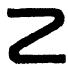
\includegraphics[keepaspectratio]{images/part003_4cdcc444.jpg}}

此外应当指出，通项为 \(u_{n}\) 的级数的收敛性对于通项因子为 \(1 + u_{n}\) 的乘积的收敛性既不必要也不充分（见习题 21 与 22）。

